\subsection{TargetScan: post-transcriptional repression burden of antigen 3'UTRs}
\label{sec:targetscan}
A tumor antigen's safety margin depends on whether normal-tissue expression
is post-transcriptionally buffered: a 3'UTR dense in conserved miRNA sites
can keep surface protein low even where RNA is detected, while an
unrepressed 3'UTR means RNA presence translates directly to surface
exposure. We audited TargetScan~8.0 default predictions (broadly conserved
miRNA families; @NHUMAN@ human genes) for all @NGENES@ study genes; a gene
absent from the table has no conserved predicted sites and is recorded as
zero burden.

\paragraph{Calibration gate.} Pre-registered gates PASSED after two recorded
first-pass miscalibrations: (G1) table depth @NHUMAN@ human genes (first-pass
threshold 15,000 failed at 13,037; the default table is narrower than the
all-predictions build); (G2) all @NGENES@ genes resolved; (G3) the HMGA2
sentinel carries conserved let-7 (GAGGUAG) sites (observed @GATETHREE@),
after two rejected control choices recorded in the audit JSON: essential
housekeeping genes (POLR2A/PCNA carry zero conserved sites, consistent with
short-UTR biology) and KRAS--let-7 (KRAS let-7 sites are not
vertebrate-conserved, and TargetScan is conservation-based).

\paragraph{Burden gated versus background.} Genes carrying at least one
conserved site: @H1G@/@H1GN@ gated versus @H1B@/@H1BN@ background (Fisher
odds ratio @H1OR@, $p=@H1P@$). Median conserved-site count @H2G@ versus
@H2B@ (Mann--Whitney $p=@H2P@$), median targeting-family breadth @H3G@
versus @H3B@ ($p=@H3P@$), and median minimum cumulative weighted context++
score @H4G@ versus @H4B@ ($p=@H4P@$). @VERDICT@

\paragraph{AND-gate antigens.} @ANTIGENBLOCK@

\begin{figure}[t]
\centering
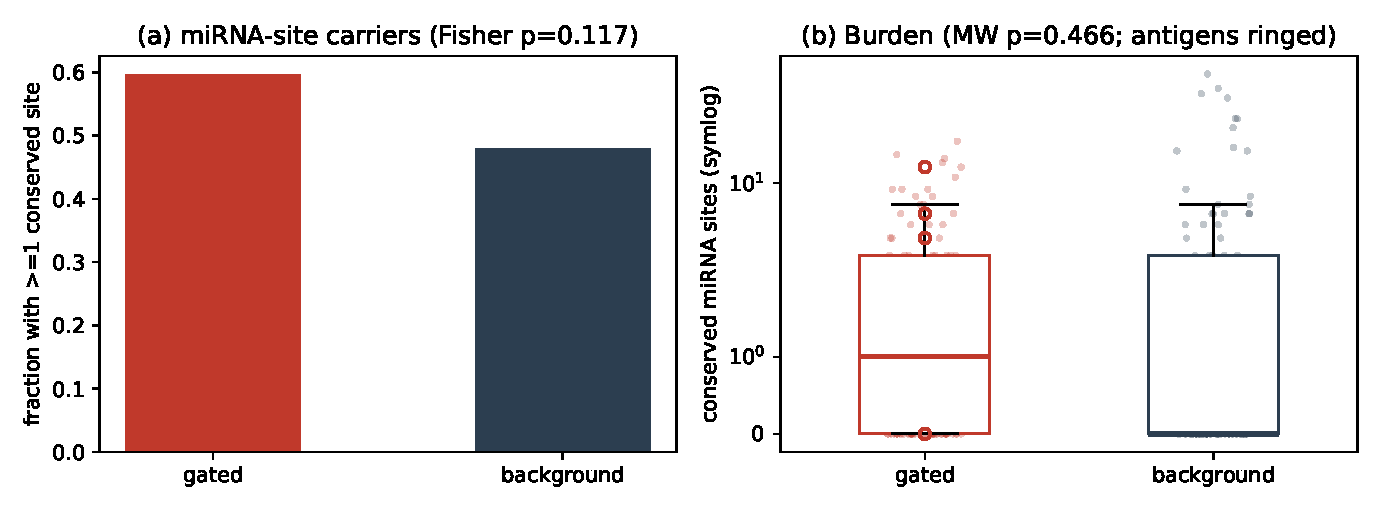
\includegraphics[width=\linewidth]{targetscan_fig.pdf}
\caption{TargetScan miRNA regulatory-burden audit. (a) Fraction of genes
carrying at least one conserved miRNA site. (b) Conserved-site burden per
gene (symlog axis), with the seven AND-gate antigens ringed.}
\label{fig:targetscan}
\end{figure}
